\begin{frame}
\frametitle{$\Higgs\to\tau\tau$?}
\begin{minipage}[c]{.3\textwidth}
\begin{center}
\begin{tikzpicture}
\draw (0,0) node (h) {\Higgs, \HiggsA};

\draw [-latex, CERNblue, thick] (h)--+(150:1.5) coordinate (u);
\draw [-latex, CERNblue, thick] (h)--+(30:1.5) coordinate (d);
\draw [-latex, CERNblue, thick] (h)--+(-90:1.5) coordinate (v);

\draw (u) node [above] (f) {fermions} ;
\draw (f) node [above] (u) {up-type} ;
\draw (d) node [above] (f) {fermions} ;
\draw (f) node [above] (d) {down-type} ;
\draw (v) node [below] (v) {vector bosons} ;

\draw [fill=red] (d.east)+(.125,.25) circle (3pt);
\draw [fill=blue] (d.east)+(.125,0) circle (3pt);
\draw [fill=ltcoloryellow] (d.east)+(.125,-.25) circle (3pt);
\draw [fill=green] (u.east)+(.125,0) circle (3pt);
\draw [fill=Burlywood4] (v.east)+(.125,0) circle (3pt);
\end{tikzpicture}
\end{center}
\end{minipage}
\hfill
\begin{minipage}[c]{.3\textwidth}
\begin{center}
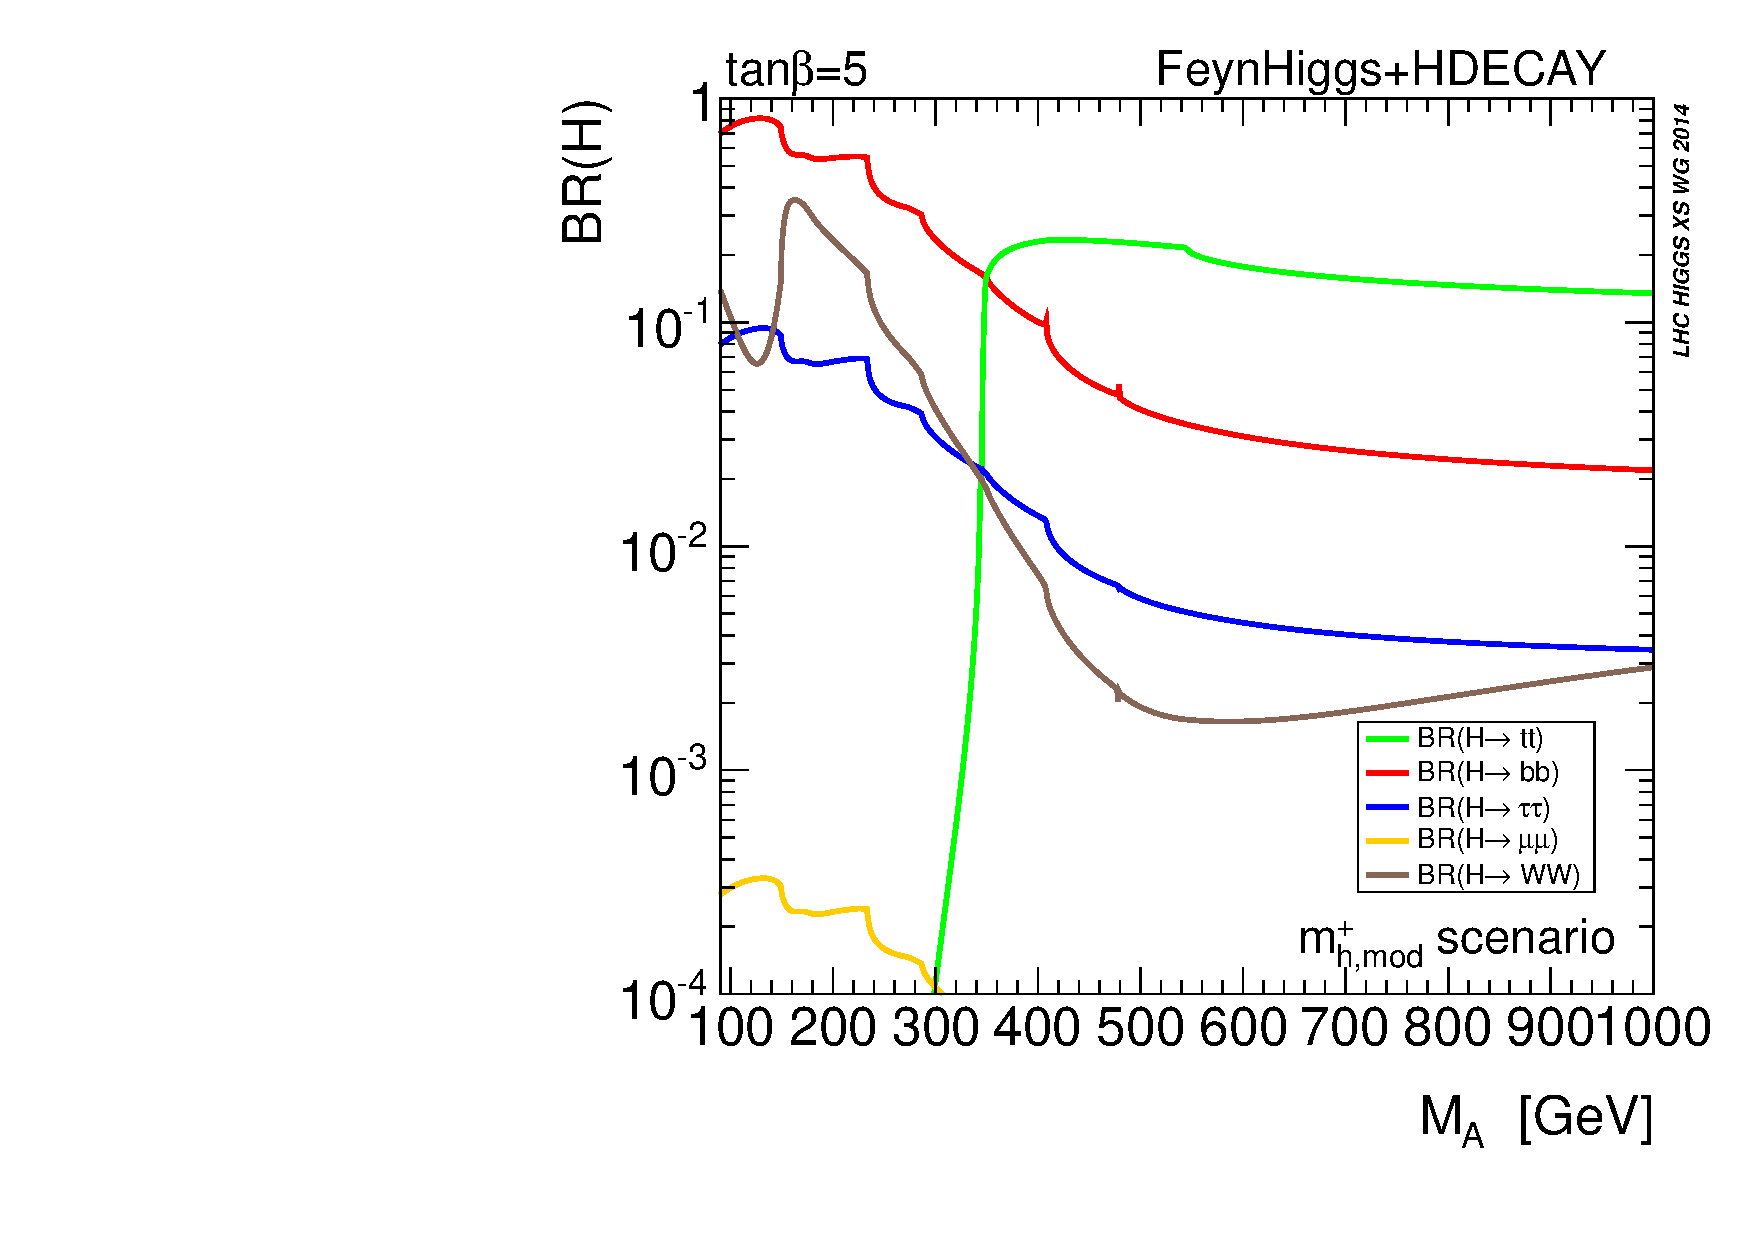
\includegraphics[width=\linewidth]{\PhDthesisdir/plots_and_images/from_Higgs_xsec_book_3/YR4HXS_BRSummary_H_mhmodp_tanbeta5_FeynHiggs_HDecay.pdf}
\end{center}
\end{minipage}
\hfill
\begin{minipage}[c]{.3\textwidth}
\begin{center}
%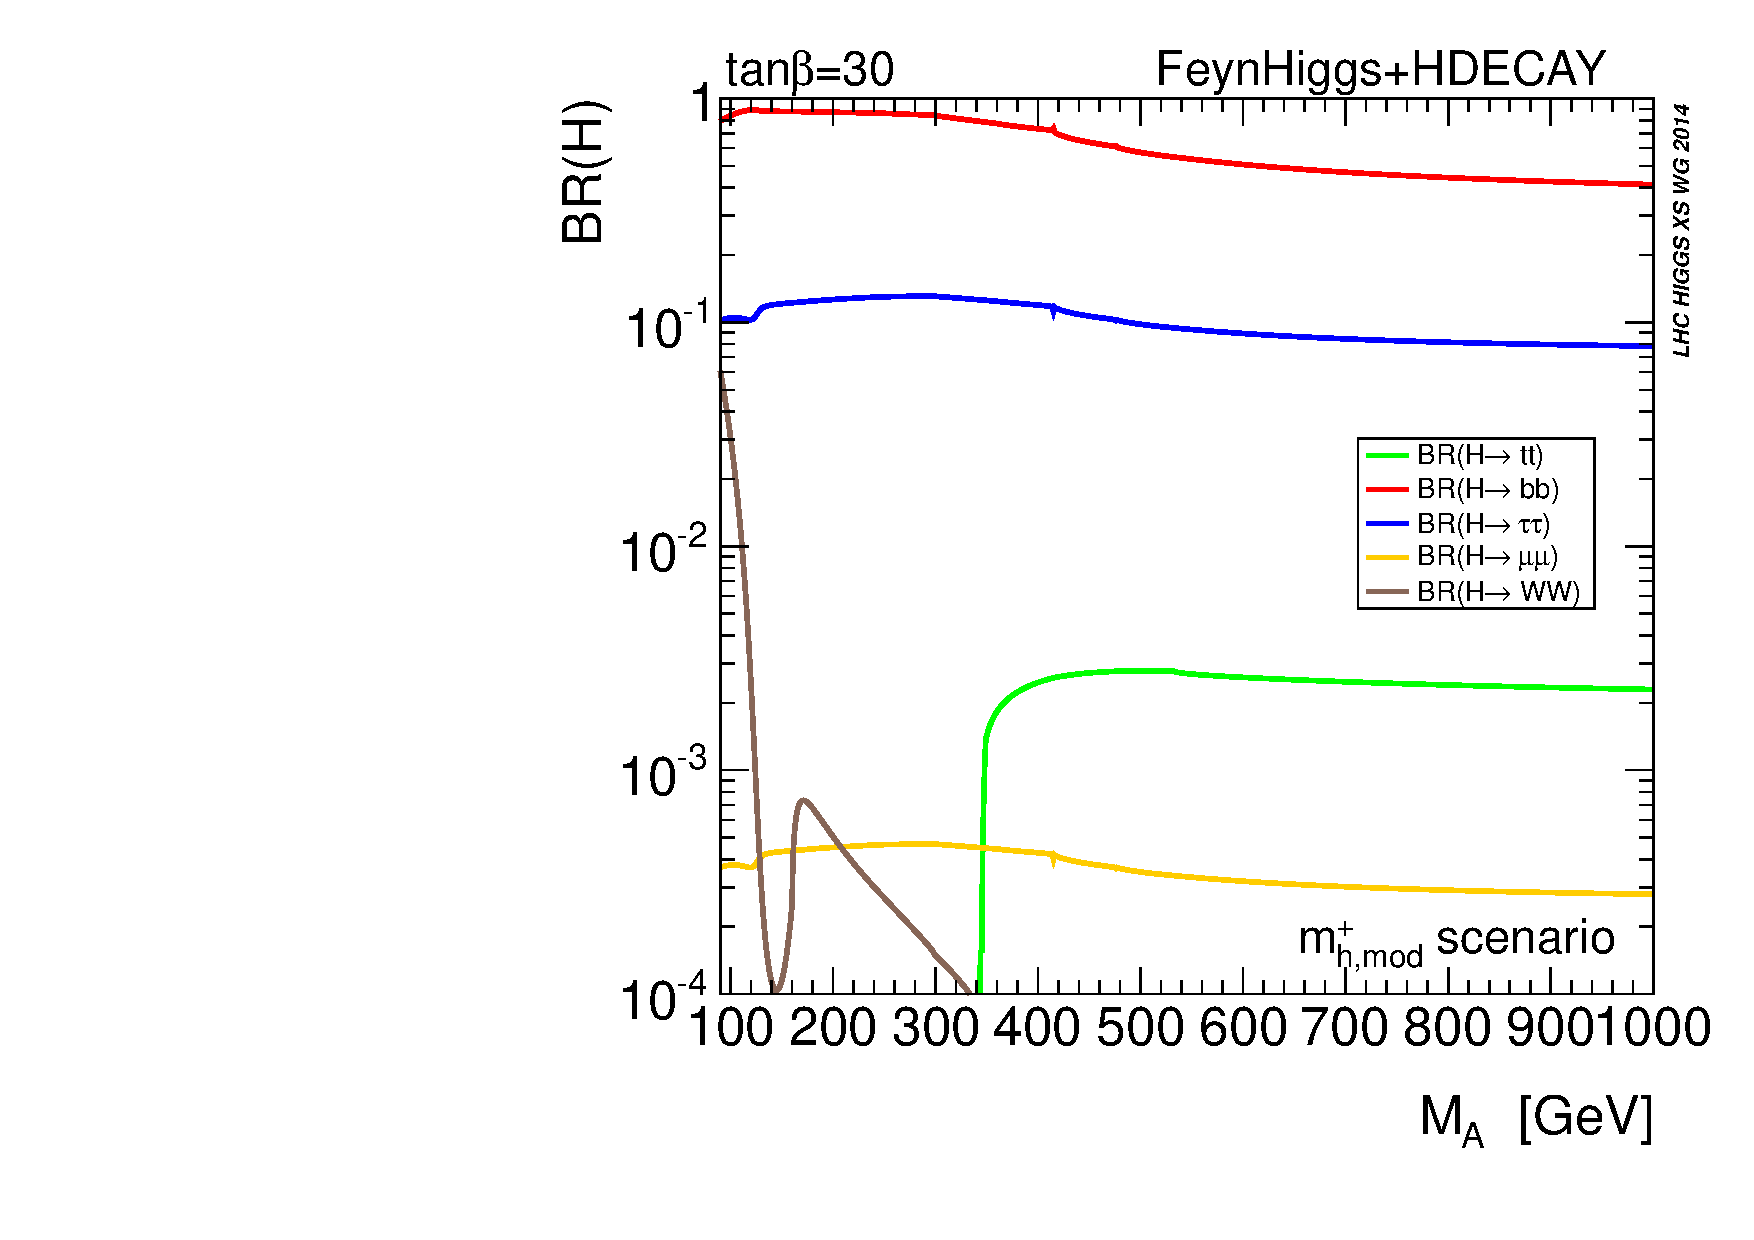
\includegraphics[width=\linewidth]{\PhDthesisdir/plots_and_images/from_Higgs_xsec_book_3/YR4HXS_BRSummary_H_mhmodp_tanbeta30_FeynHiggs_HDecay.pdf}
\end{center}
\end{minipage}
%\manip Looking for a trace of additionnal Higgs: what do they decay into?
\beamercite{CMS-PAS-HIG-17-020}
\beamercite{Higgs_xsec_book_3}
\end{frame}

%At leading-order (LO), the coupling of the \Higgs\ and the \HiggsA\ to down-type fermions is enhanced by $\tan\beta$ with respect to the expectation for an SM Higgs boson of the same mass, while the coupling to vector bosons and up-type fermions is suppressed.

\begin{frame}\addtocounter{framenumber}{-1}
\frametitle{$\Higgs\to\tau\tau$? -- enhanced and suppressed couplings}
\begin{minipage}[c]{.3\textwidth}
\begin{center}
\begin{tikzpicture}
\draw (0,0) node (h) {\Higgs, \HiggsA};

\draw [-latex, CERNblue, thick, dashed] (h)--+(150:1.5) coordinate (u);
\draw [-latex, CERNblue, thick] (h)--+(30:1.5) coordinate (d);
\draw [-latex, CERNblue, thick, dashed] (h)--+(-90:1.5) coordinate (v);

\draw [ltcolorgray2] (u) node [above] (f) {fermions} ;
\draw [ltcolorgray2] (f) node [above] (u) {up-type} ;
\draw (d) node [above] (f) {fermions} ;
\draw (f) node [above] (d) {down-type} ;
\draw [ltcolorgray2] (v) node [below] (v) {vector bosons} ;

\draw [fill=red] (d.east)+(.125,.25) circle (3pt);
\draw [fill=blue] (d.east)+(.125,0) circle (3pt);
\draw [fill=ltcoloryellow] (d.east)+(.125,-.25) circle (3pt);
\draw [fill=green] (u.east)+(.125,0) circle (3pt);
\draw [fill=Burlywood4] (v.east)+(.125,0) circle (3pt);

\draw (30:.75) node [right] {\ $\times\tan\beta$};
\end{tikzpicture}
\end{center}
\end{minipage}
\hfill
\begin{minipage}[c]{.3\textwidth}
\begin{center}
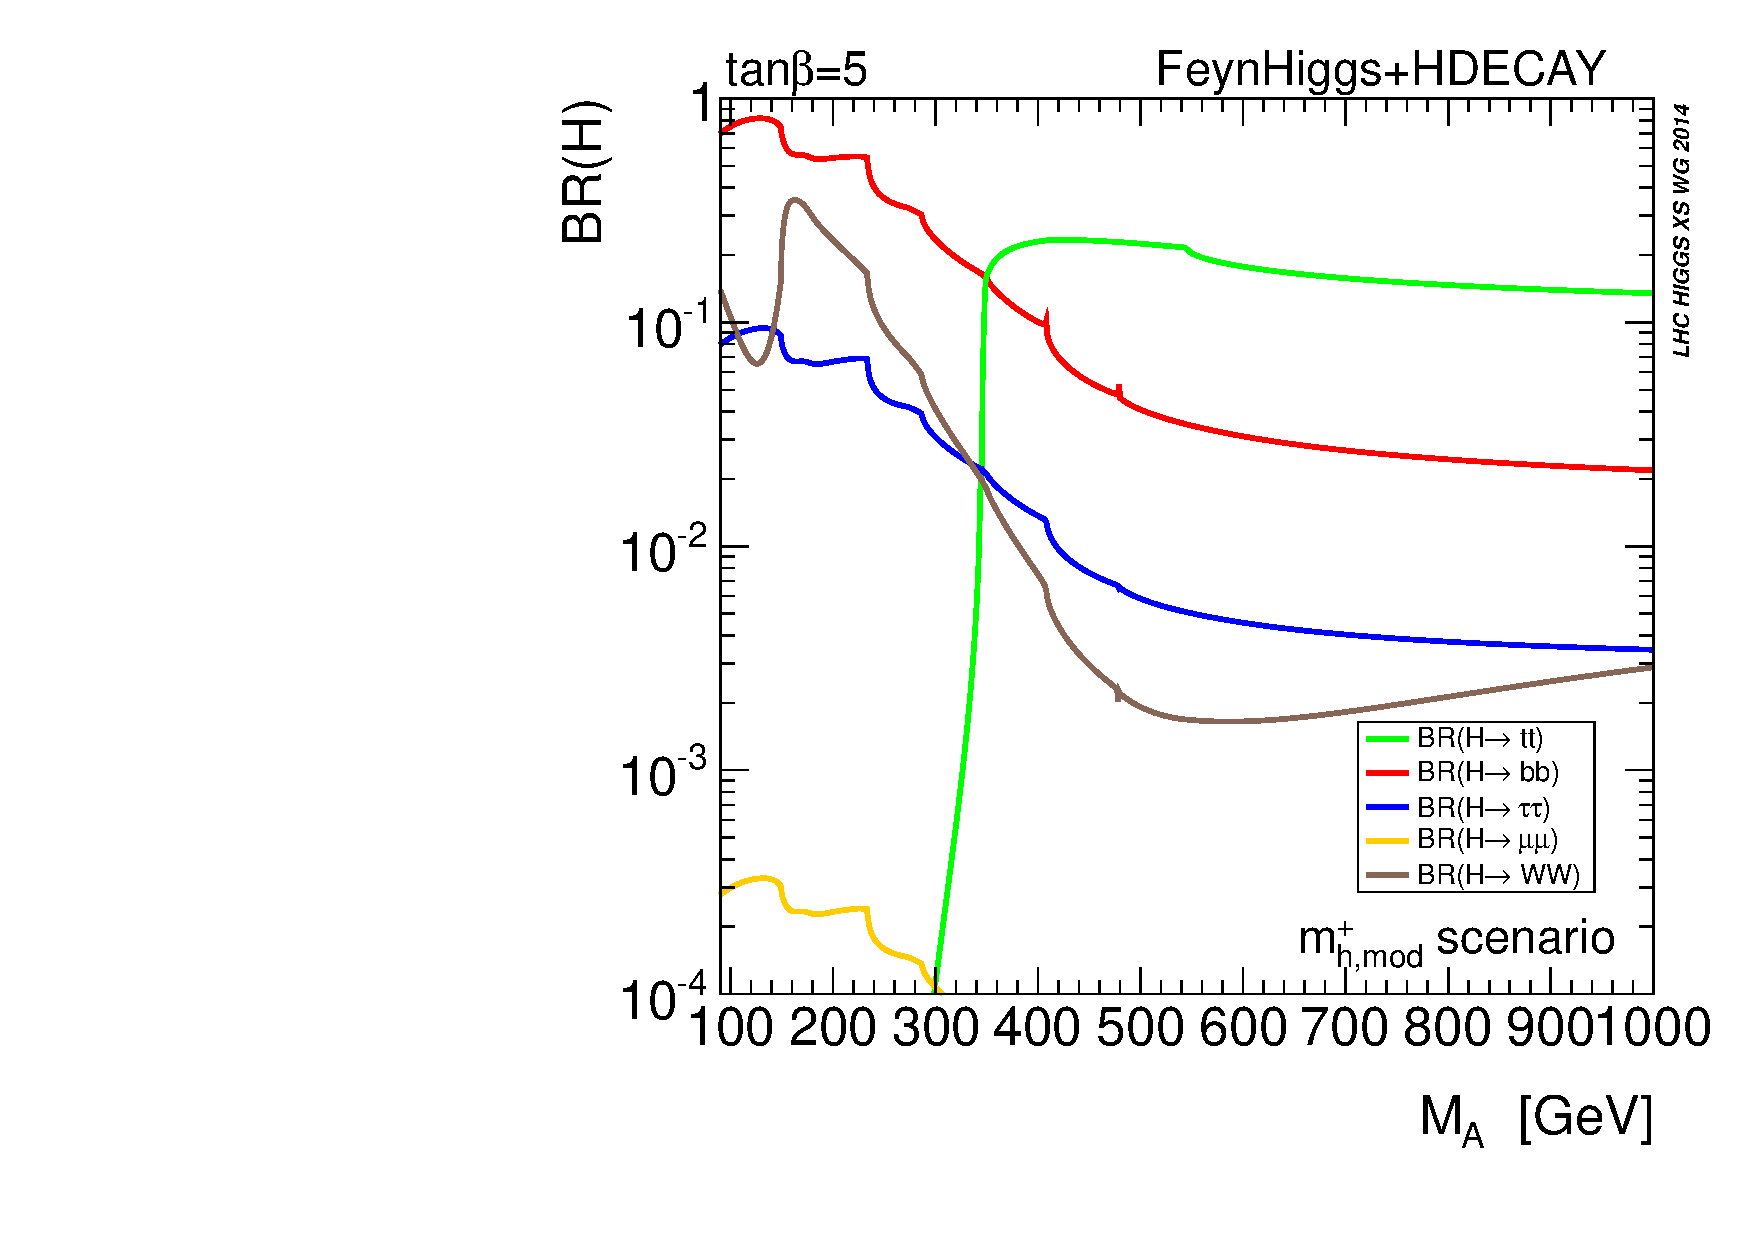
\includegraphics[width=\linewidth]{\PhDthesisdir/plots_and_images/from_Higgs_xsec_book_3/YR4HXS_BRSummary_H_mhmodp_tanbeta5_FeynHiggs_HDecay.pdf}
\end{center}
\end{minipage}
\hfill
\begin{minipage}[c]{.3\textwidth}
\begin{center}
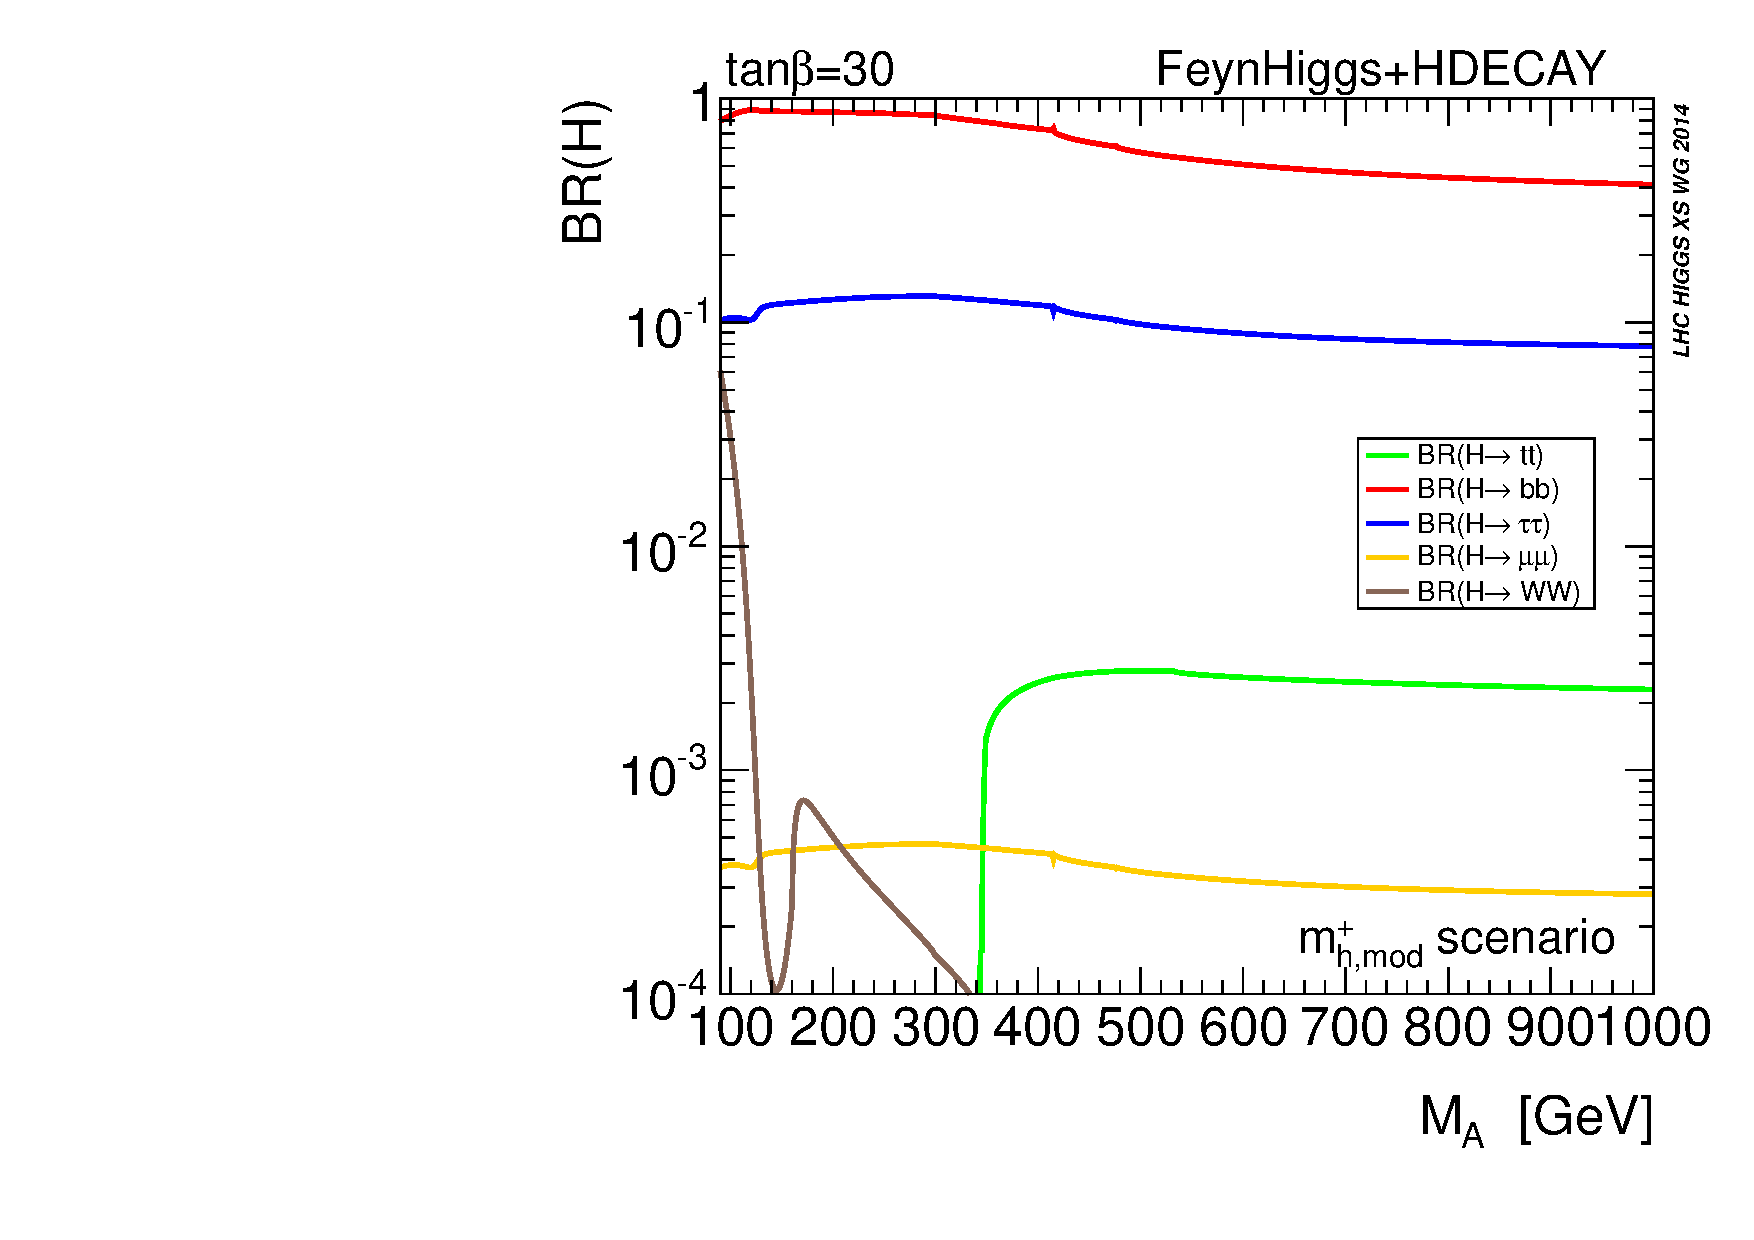
\includegraphics[width=\linewidth]{\PhDthesisdir/plots_and_images/from_Higgs_xsec_book_3/YR4HXS_BRSummary_H_mhmodp_tanbeta30_FeynHiggs_HDecay.pdf}
\end{center}
\end{minipage}
%\manip At high $\tan\bet$, some couplings are suppressed, other enhanced by $\tan\beta$.
\beamercite{CMS-PAS-HIG-17-020}
\beamercite{Higgs_xsec_book_3}
\end{frame}

\begin{frame}
\frametitle{$\Higgs\to\tau\tau$?}
\begin{minipage}[c]{.3\textwidth}
\begin{center}
\begin{tikzpicture}
\draw (0,0) node (h) {\Higgs, \HiggsA};
\foreach \coord/\ptc/\txtcolor/\width/\dash/\angle in {
ele/$\antielectron\electron$/ltcolorgray2/very thin//120,
mu/$\antimuon\muon$/ltcolorgray2///60,
tau/$\antitau\leptau$//very thick//0,
d/$\quarkd\antiquarkd$/ltcolorgray2/ultra thin//-60,
s/$\quarks\antiquarks$/ltcolorgray2///-120,
b/$\quarkb\antiquarkb$//ultra thick//-180}{
\draw [-latex, CERNblue, thick] (h)--+(\angle:1.35) ;
\draw (h)+(\angle:1.75) node (\coord) {\ptc} ;
\draw (\coord) node {\vphantom{\LARGE ÀQ}} ;
}

\draw [fill=red] (b.south) circle (3pt);
\draw [fill=blue] (tau.south) circle (3pt);
\draw [fill=ltcoloryellow] (mu.south) circle (3pt);
\end{tikzpicture}
\end{center}
\end{minipage}
\hfill
\begin{minipage}[c]{.3\textwidth}
\begin{center}
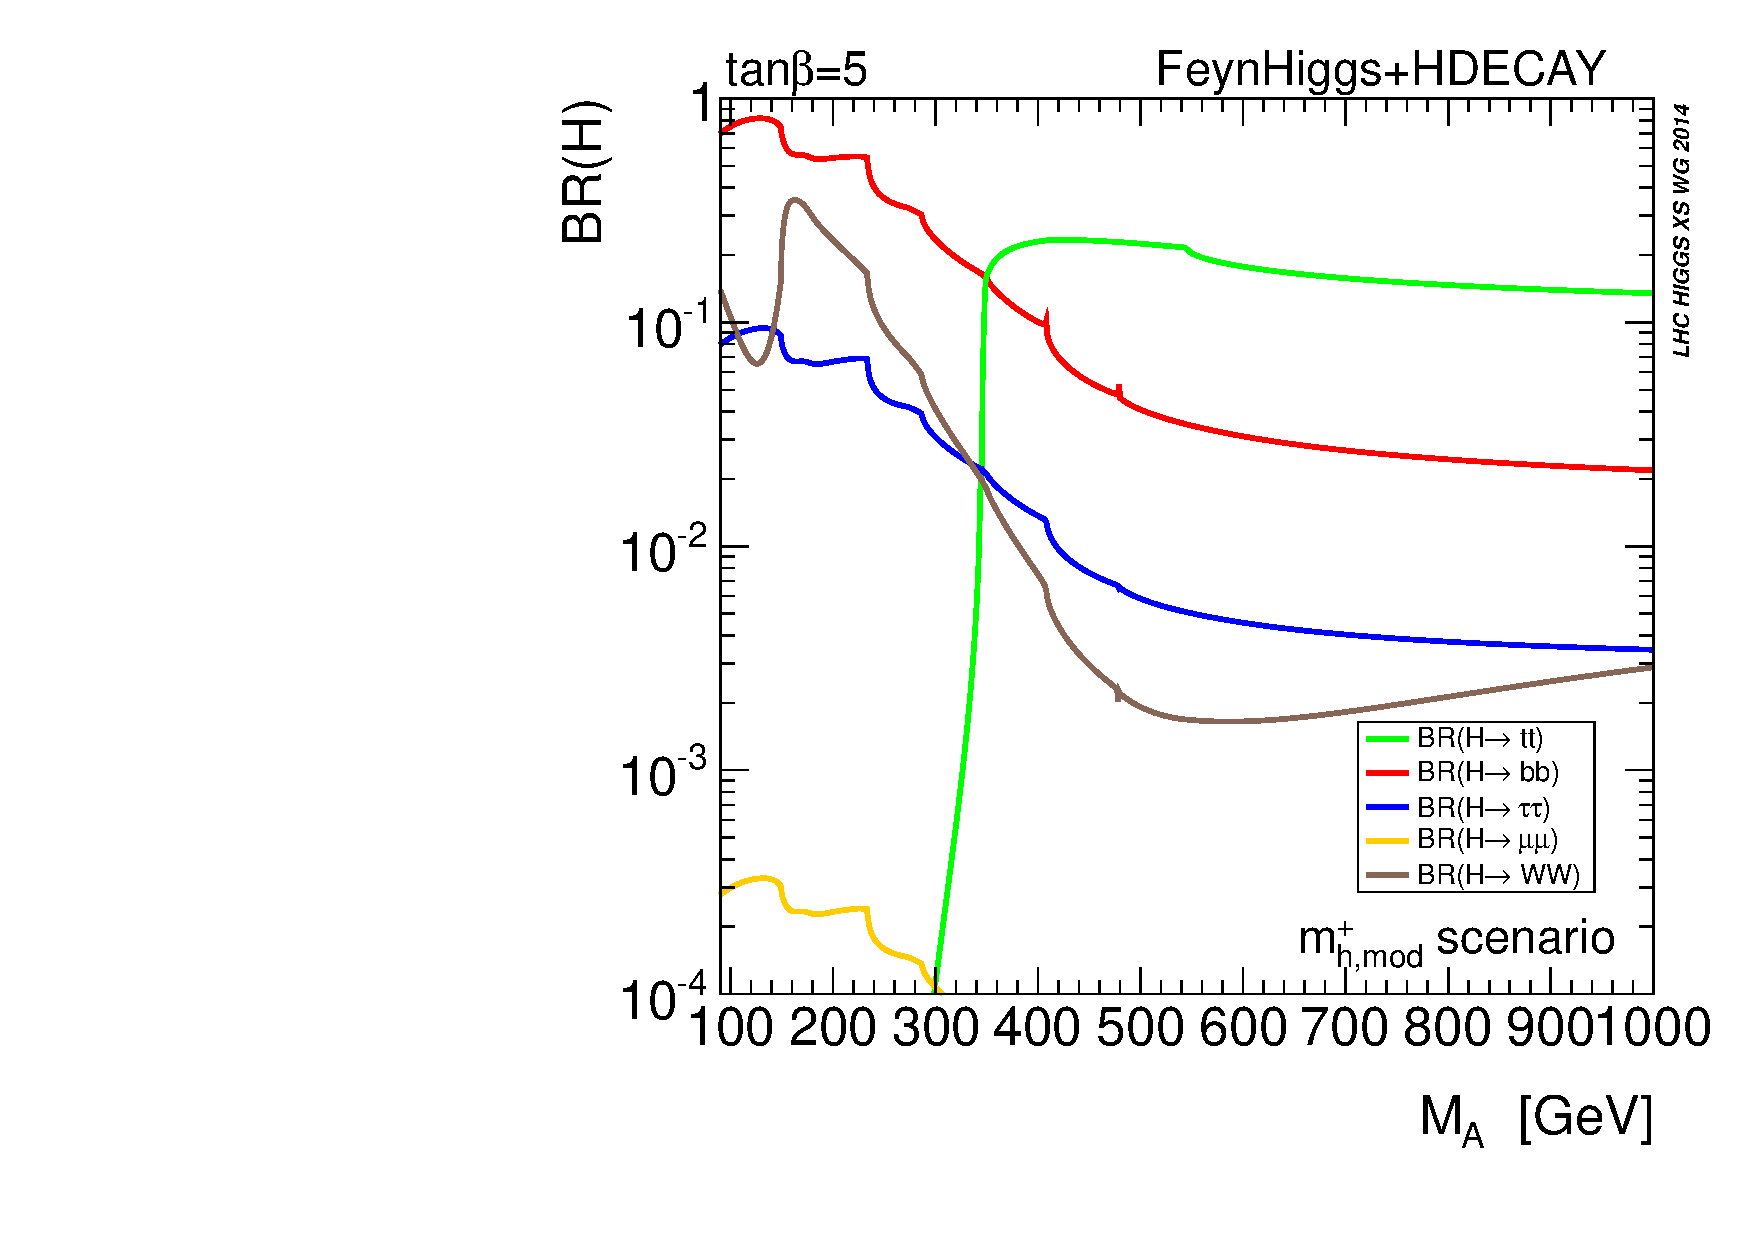
\includegraphics[width=\linewidth]{\PhDthesisdir/plots_and_images/from_Higgs_xsec_book_3/YR4HXS_BRSummary_H_mhmodp_tanbeta5_FeynHiggs_HDecay.pdf}
\end{center}
\end{minipage}
\hfill
\begin{minipage}[c]{.3\textwidth}
\begin{center}
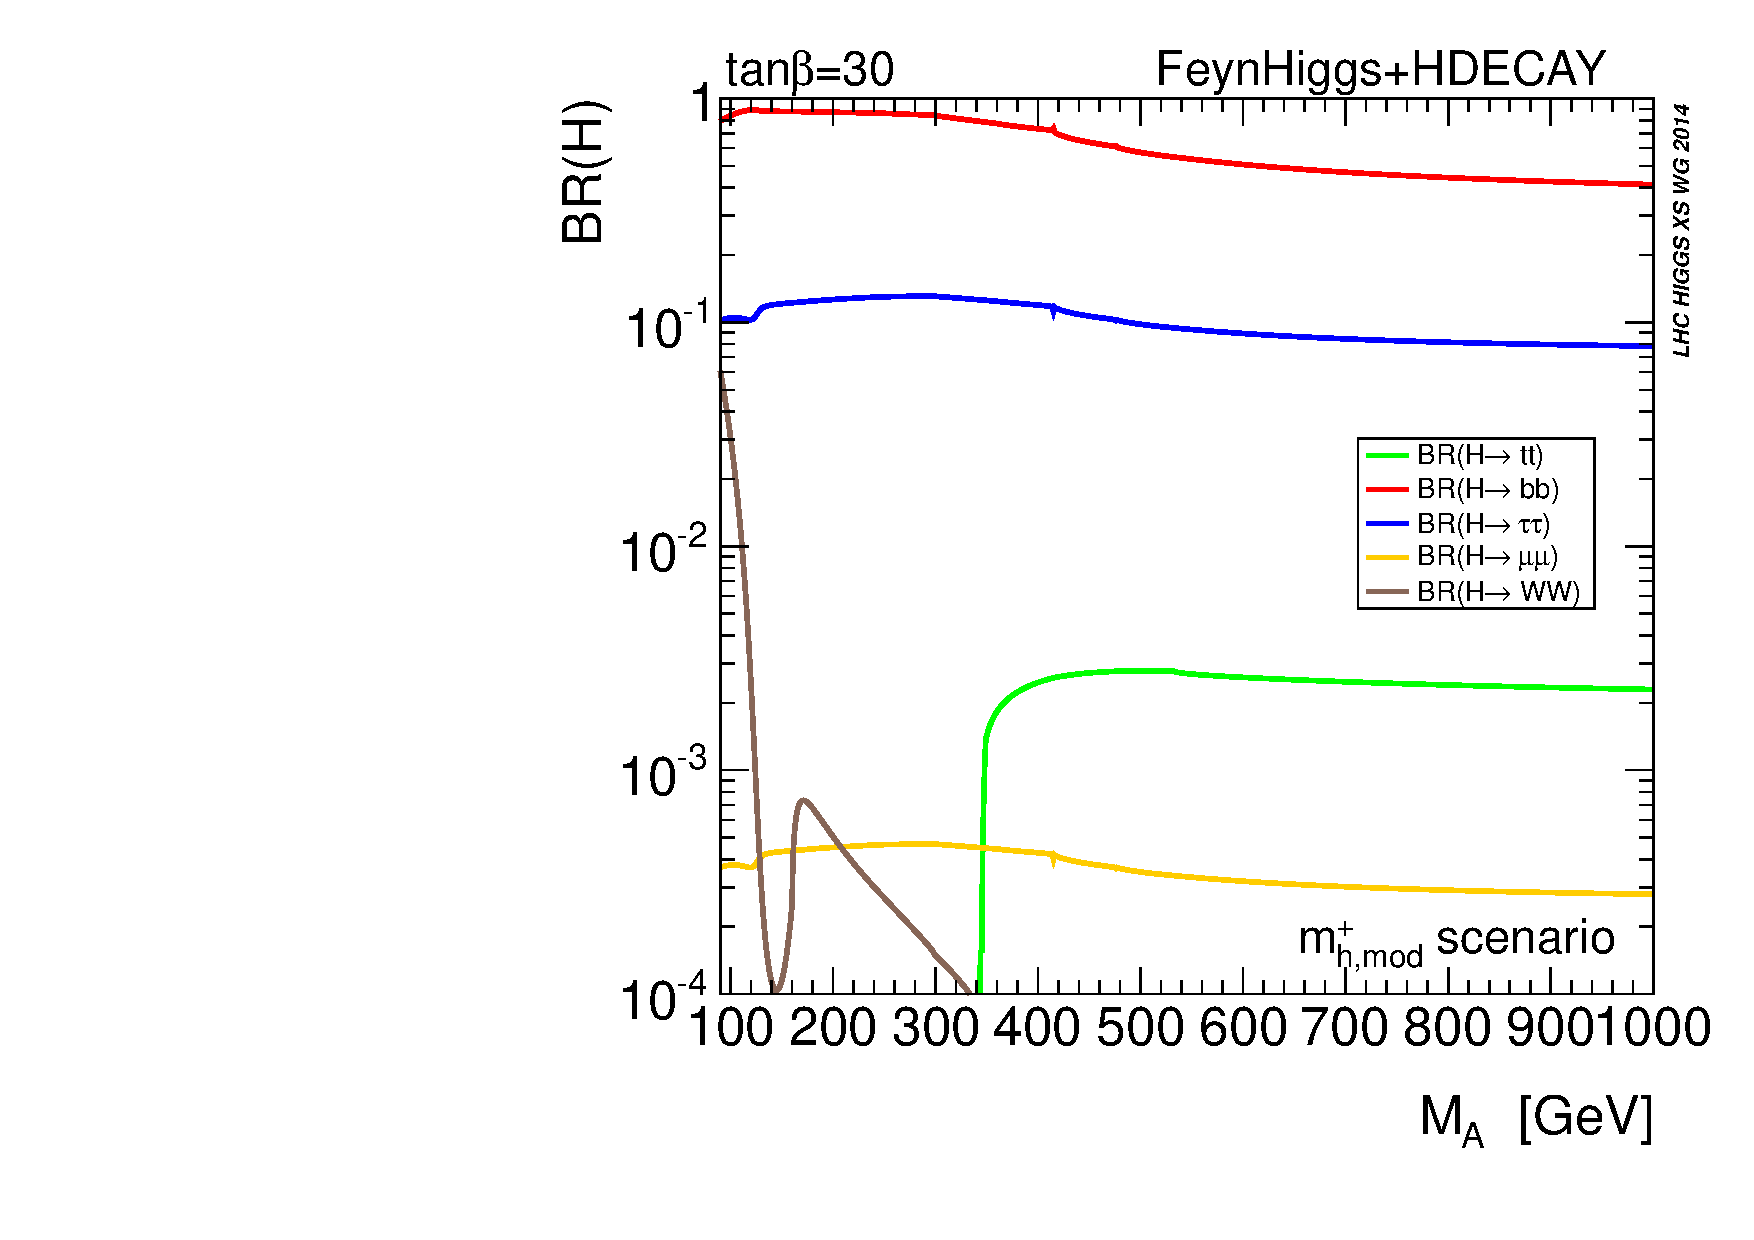
\includegraphics[width=\linewidth]{\PhDthesisdir/plots_and_images/from_Higgs_xsec_book_3/YR4HXS_BRSummary_H_mhmodp_tanbeta30_FeynHiggs_HDecay.pdf}
\end{center}
\end{minipage}
\beamercite{CMS-PAS-HIG-17-020}
\beamercite{Higgs_xsec_book_3}
\end{frame}

\begin{frame}\addtocounter{framenumber}{-1}
\frametitle{$\Higgs\to\tau\tau$? -- Higgs couplings and particules masses}
\begin{minipage}[c]{.3\textwidth}
\begin{center}
\begin{tikzpicture}
\draw (0,0) node (h) {\Higgs, \HiggsA};
\foreach \coord/\ptc/\txtcolor/\width/\dash/\angle in {
ele/$\antielectron\electron$/ltcolorgray2/very thin//120,
mu/$\antimuon\muon$/ltcolorgray2///60,
tau/$\antitau\leptau$//very thick//0,
d/$\quarkd\antiquarkd$/ltcolorgray2/ultra thin//-60,
s/$\quarks\antiquarks$/ltcolorgray2///-120,
b/$\quarkb\antiquarkb$//ultra thick//-180}{
\draw [-latex, CERNblue, \width] (h)--+(\angle:1.35) ;
\draw [\txtcolor] (h)+(\angle:1.75) node (\coord) {\ptc} ;
\draw (\coord) node {\vphantom{\LARGE ÀQ}} ;
}

\draw [fill=red] (b.south) circle (3pt);
\draw [fill=blue] (tau.south) circle (3pt);
\draw [fill=ltcoloryellow] (mu.south) circle (3pt);
\end{tikzpicture}
\end{center}
\end{minipage}
\hfill
\begin{minipage}[c]{.3\textwidth}
\begin{center}
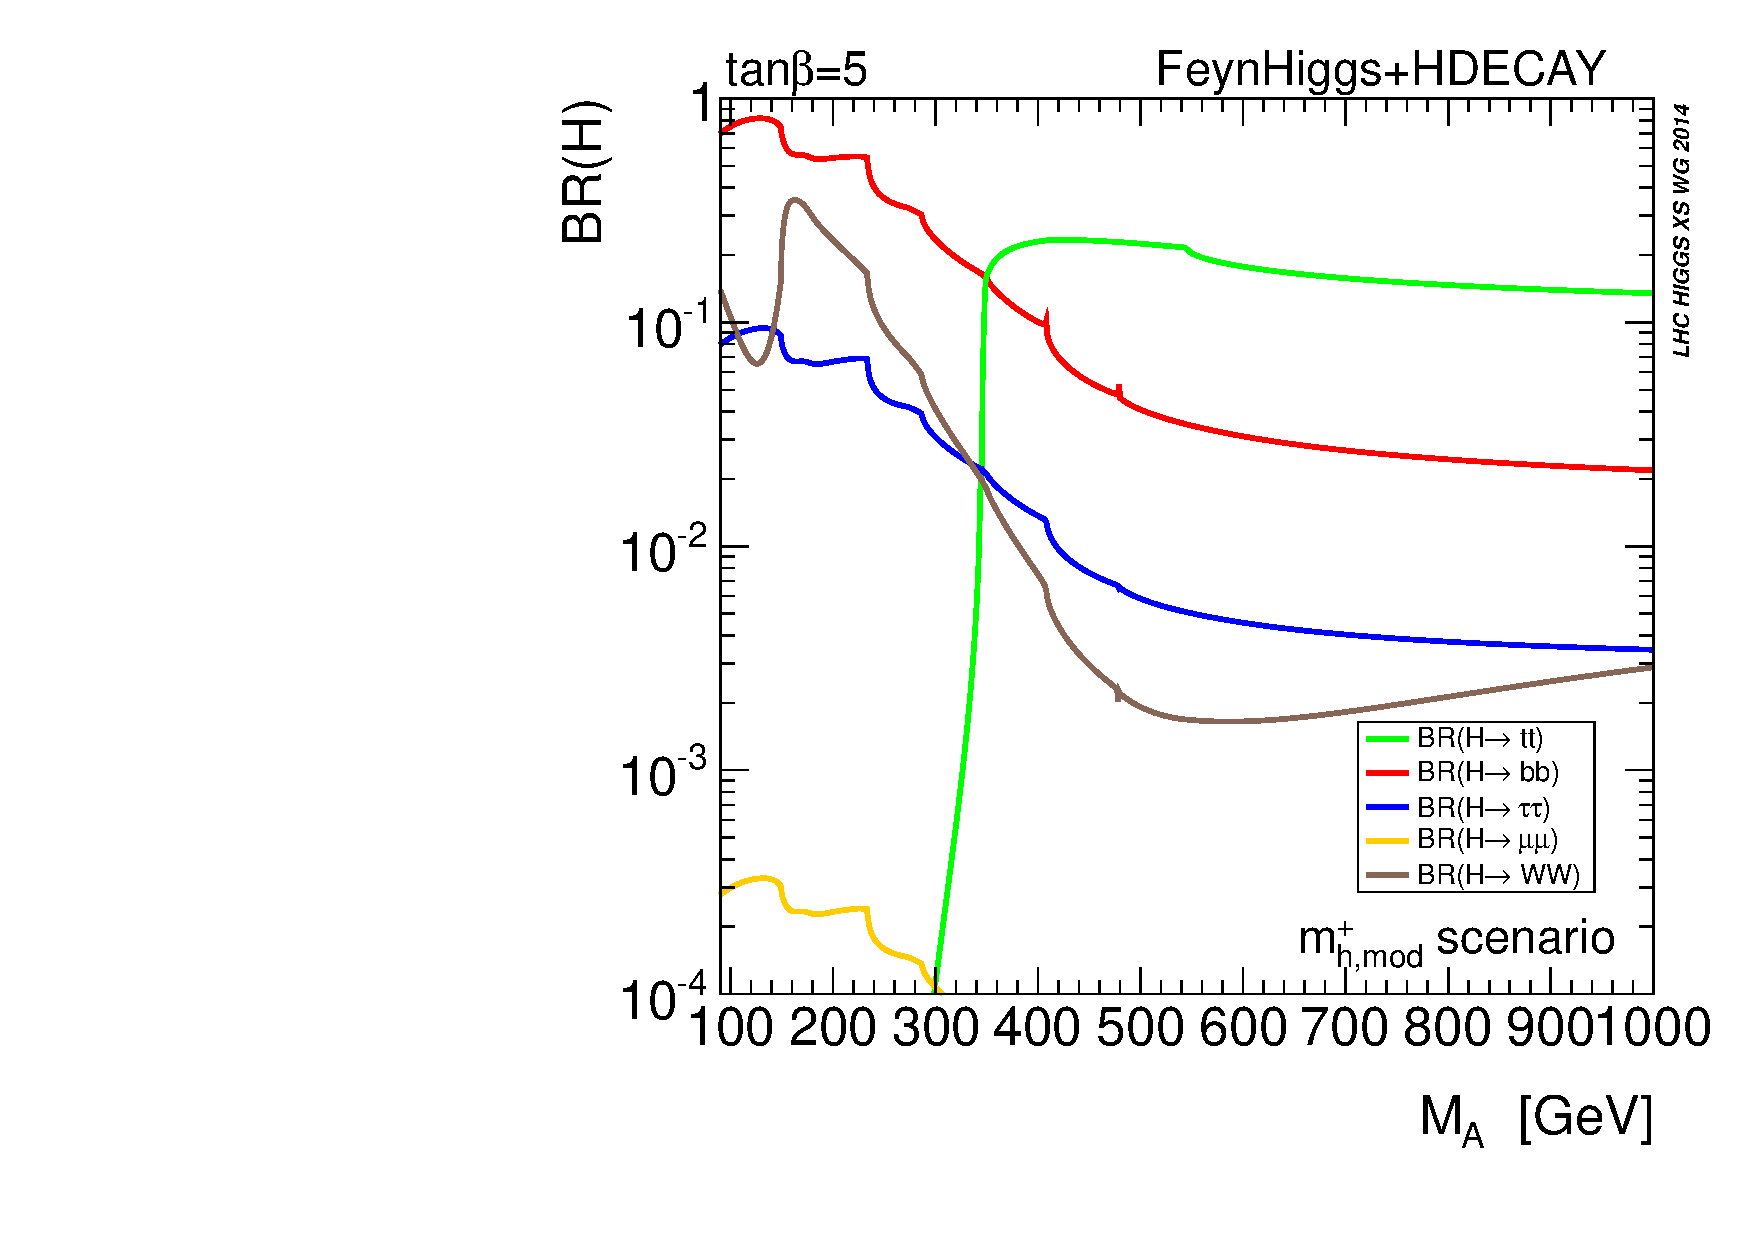
\includegraphics[width=\linewidth]{\PhDthesisdir/plots_and_images/from_Higgs_xsec_book_3/YR4HXS_BRSummary_H_mhmodp_tanbeta5_FeynHiggs_HDecay.pdf}
\end{center}
\end{minipage}
\hfill
\begin{minipage}[c]{.3\textwidth}
\begin{center}
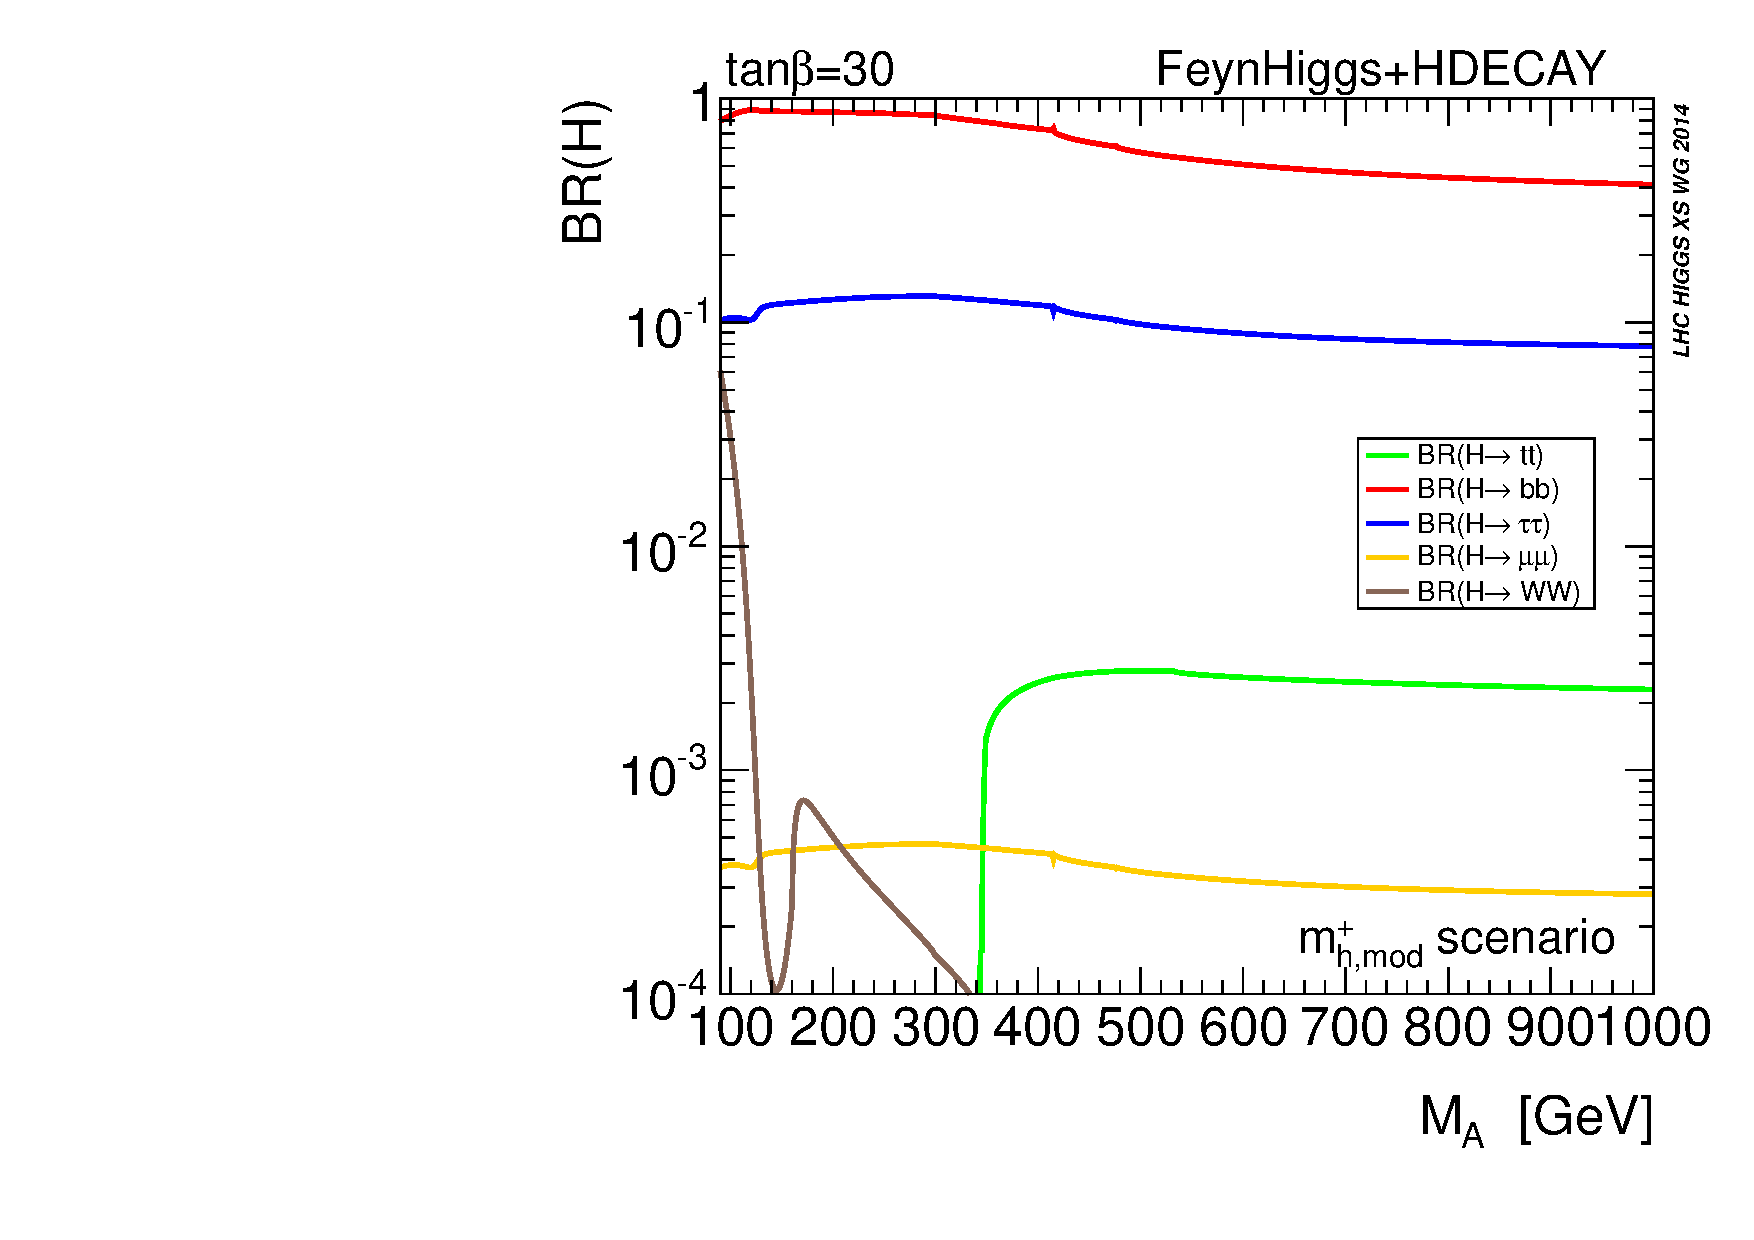
\includegraphics[width=\linewidth]{\PhDthesisdir/plots_and_images/from_Higgs_xsec_book_3/YR4HXS_BRSummary_H_mhmodp_tanbeta30_FeynHiggs_HDecay.pdf}
\end{center}
\end{minipage}
\beamercite{CMS-PAS-HIG-17-020}
\beamercite{Higgs_xsec_book_3}
\end{frame}

\begin{frame}\addtocounter{framenumber}{-1}
\frametitle{$\Higgs\to\tau\tau$? -- avoid hadronic background}
\begin{minipage}[c]{.3\textwidth}
\begin{center}
\begin{tikzpicture}
\draw (0,0) node (h) {\Higgs, \HiggsA};
\foreach \coord/\ptc/\txtcolor/\width/\dash/\angle in {
ele/$\antielectron\electron$/ltcolorgray2/very thin//120,
mu/$\antimuon\muon$/ltcolorgray2///60,
tau/$\antitau\leptau$//very thick//0,
d/$\quarkd\antiquarkd$/ltcolorgray2/ultra thin//-60,
s/$\quarks\antiquarks$/ltcolorgray2///-120,
b/$\quarkb\antiquarkb$/ltcolorgray2/ultra thick//-180}{
\draw [-latex, CERNblue, \width, \dash] (h)--+(\angle:1.35) ;
\draw [\txtcolor] (h)+(\angle:1.75) node (\coord) {\ptc} ;
\draw (\coord) node {\vphantom{\LARGE ÀQ}} ;
}

\draw [fill=red] (b.south) circle (3pt);
\draw [fill=blue] (tau.south) circle (3pt);
\draw [fill=ltcoloryellow] (mu.south) circle (3pt);

\draw [ltcolorgreen] (tau.north) node [above] {\LARGE\bfseries \OK};
\end{tikzpicture}
\end{center}
\end{minipage}
\hfill
\begin{minipage}[c]{.3\textwidth}
\begin{center}
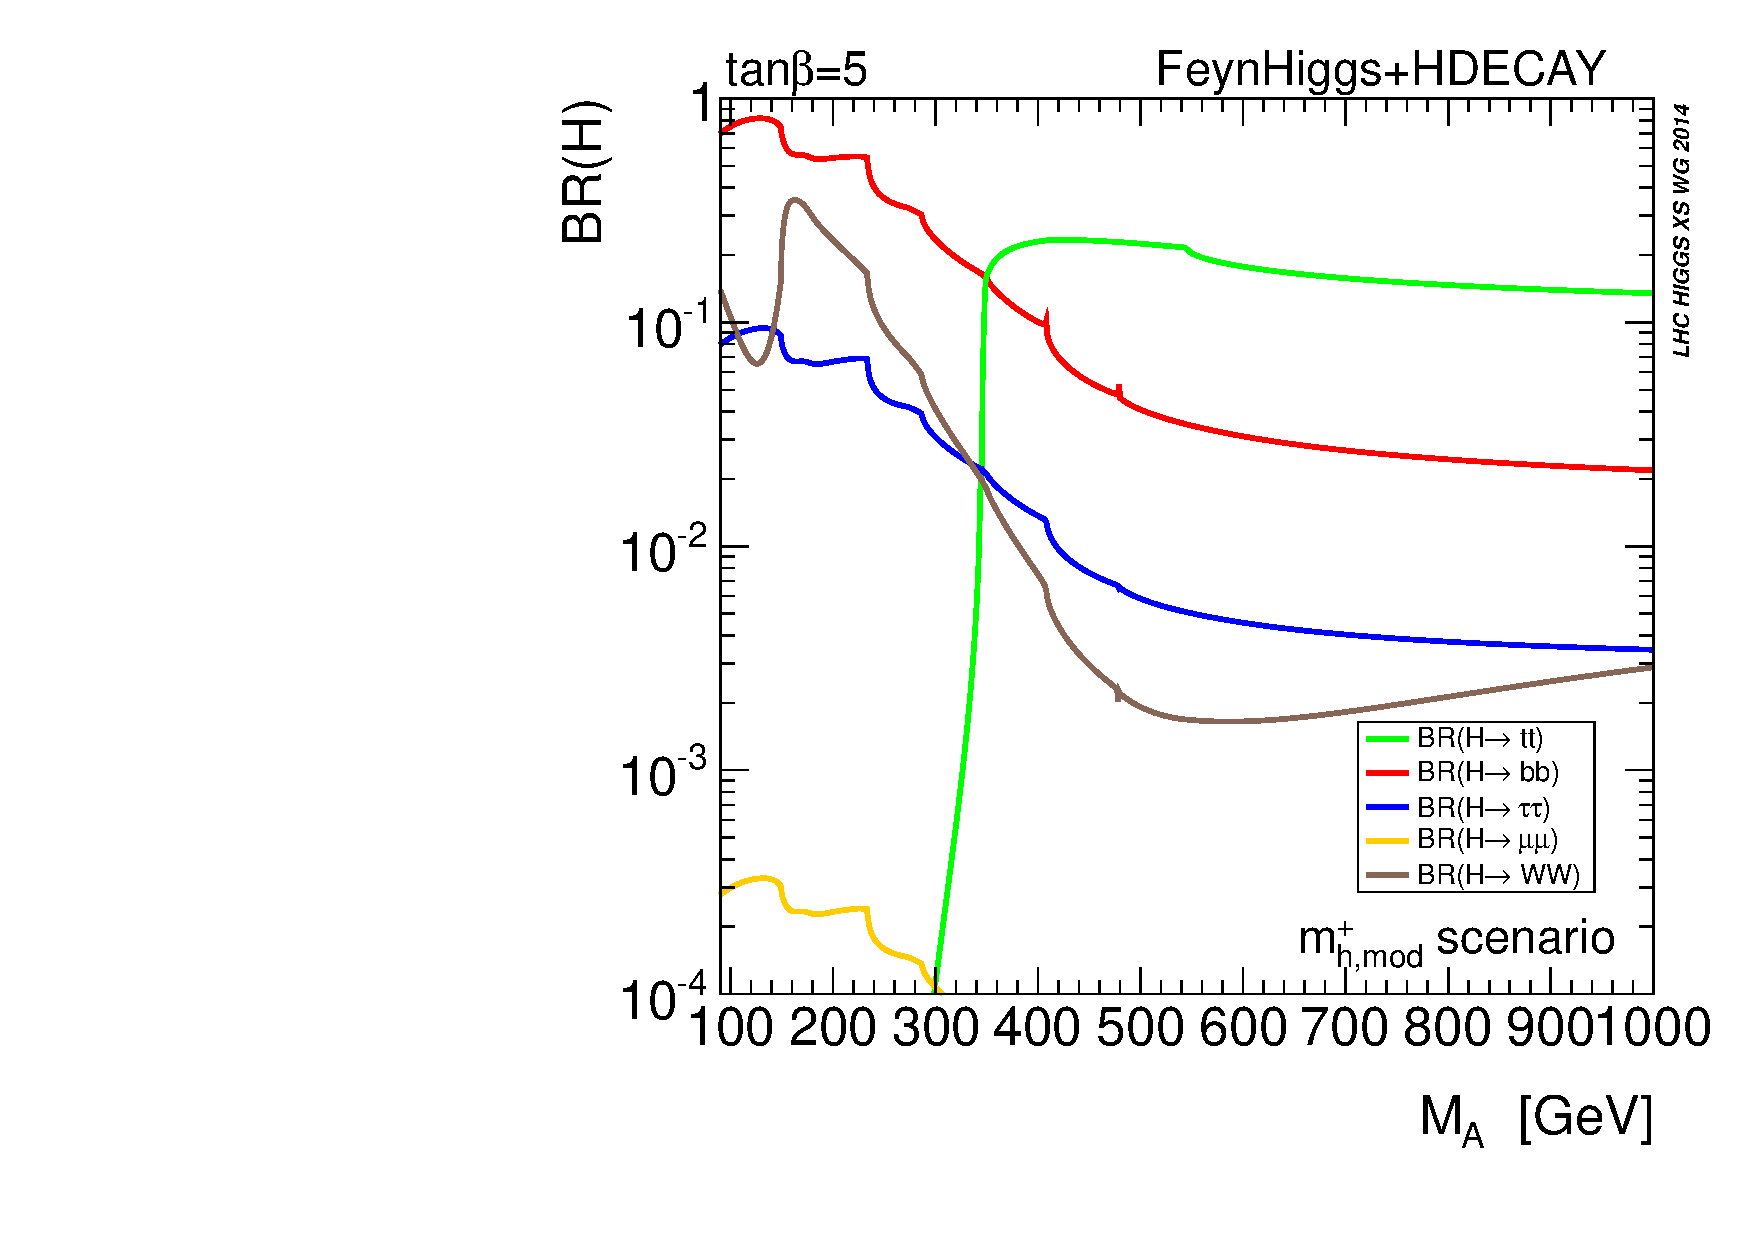
\includegraphics[width=\linewidth]{\PhDthesisdir/plots_and_images/from_Higgs_xsec_book_3/YR4HXS_BRSummary_H_mhmodp_tanbeta5_FeynHiggs_HDecay.pdf}
\end{center}
\end{minipage}
\hfill
\begin{minipage}[c]{.3\textwidth}
\begin{center}
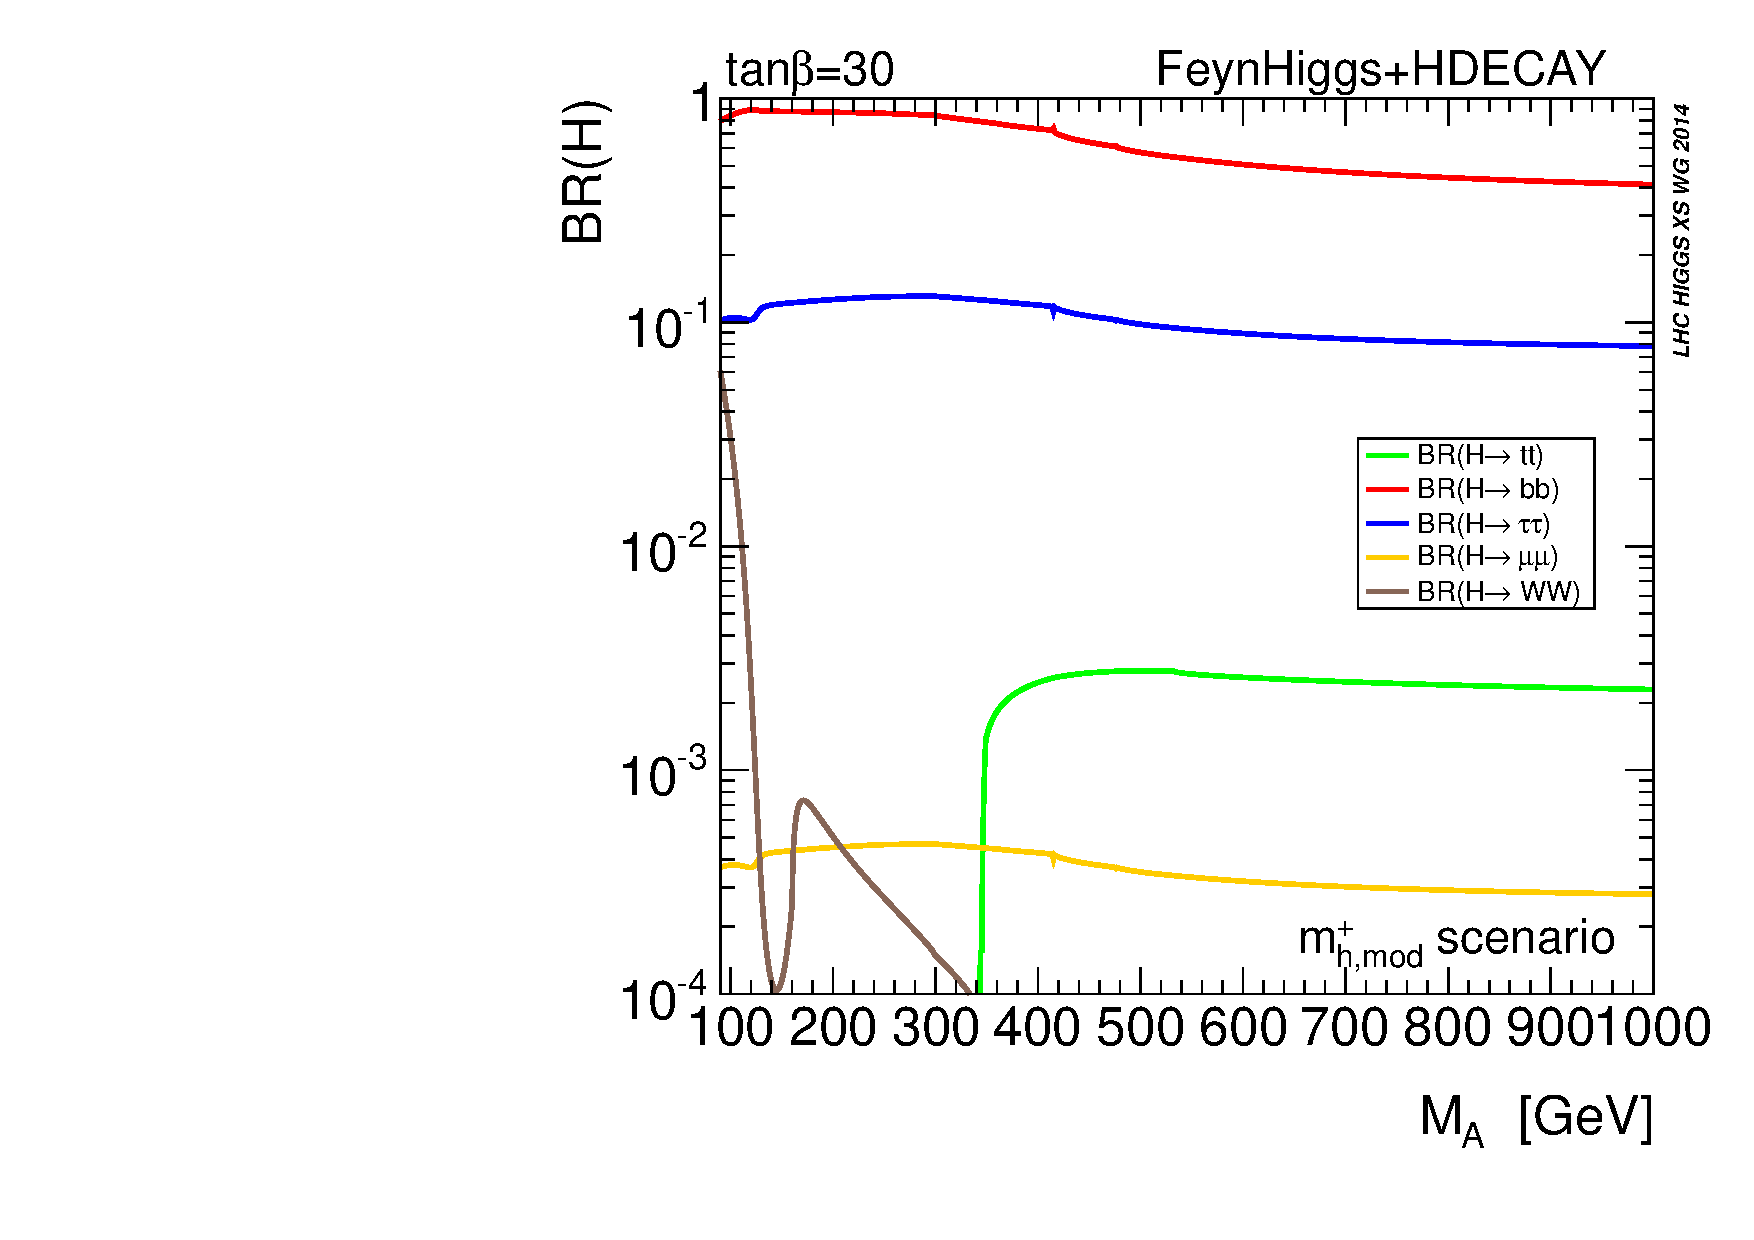
\includegraphics[width=\linewidth]{\PhDthesisdir/plots_and_images/from_Higgs_xsec_book_3/YR4HXS_BRSummary_H_mhmodp_tanbeta30_FeynHiggs_HDecay.pdf}
\end{center}
\end{minipage}
\beamercite{CMS-PAS-HIG-17-020}
\beamercite{Higgs_xsec_book_3}
\end{frame}
